\section{Results and discussion}

\revise{}{
\subsection{Printing results}
In order to accurately manufacture adaptive width toolpaths using an off-the-shelf 3D printing system.
we need a model which relates the required width to process parameters such as movement speed and filament extrusion speed.
A different approach might be appropriate depending on whether the filament feeder is mounted directly on the print head (a.k.a. \emph{direct drive}) or the filament fed from the back of the printer to the print head via a \emph{Bowden tube}.
Because Bowden style 3D printing systems have the filament feeder relatively far away from the nozzle changing the internal pressure in the system requires a large amount of filament movement, which requires a prohibitive amount of time.

\paragraph{Back pressure compensation}
We therefore keep the internal pressure constant, and vary the movement speed instead.
%In order to accurately realize a varying bead width we vary the movement speed, while keeping the internal pressure in the system constant.
One approach would be keep the filament inflow $f$ (in \si{\milli\meter\cubed\per\second}) constant by varying movement speed accordingly \cite{Kuipers2018}.
However, that doesn't result in the intended filament outflow variation - see \cref{zero_back_pressure}.
We conjecture that the filament outflow is related to the total pressure in the system,
which depends not only on the amount of filament in between the feeder wheel and the nozzle (which we keep constant), 
but also depends on the back pressure that the previous layer exerts on the filament protruding from the nozzle.
We conjecture that the amount of back pressure is monotonically related to the requested line width and compensate for the back pressure using a simple linear model:

\begin{align}
 v(w) &= \frac{f(w)}{h w} \\ 
% f &\sim p \\
% p &= p_\text{in} + p_\text{ext} \\
% p_\text{in} &= C \\
% p_\text{ext} &\sim w \\
% p_\text{ext} &= w / w^* - 1 \\
% f &= f^* - k p_\text{ext} \\
 f(w) &= f_0 - k \left( w / w_0 - 1 \right) \\
 f_0 &= v_0 w_0 h 
% v &= \frac{f^* - k p_\text{ext}}{h w} \\ 
% v &= \frac{v^* w^* h - k (w / w^* - 1)}{h w}
\end{align}
where
$v(w)$ is the movement speed as a function of requested bead width $w$,
$f(w)$ is the filament outflow,
$f_0$ is a constant reference flow
and
$k$ is the amount of back pressure compensation.
Using increments of $0.1$ we established that using a factor of $k=1.1$ yields satisfactory bead width variation for our setup where
$v_0=\SI{30}{\milli\meter\per\second}$, 
$w_0=\SI{0.4}{\milli\meter}$.
See \cref{back_pressure}.
The fact that the printed lines are wider than intended is compensated for using a flow reduction to \SI{90}{\percent}.
%
Test prints were performed on an unmodified Ultimaker S5 system,
with a standard  \SI{0.4}{\milli\meter} nozzle
and PLA filament
and a layer thickness of $h=\SI{0.1}{\milli\meter}$.
Because the machine instructions file format \emph{G-code} doesn't natively support adaptive width beads,
we discretize adaptive width extrusions into \SI{0.2}{\milli\meter} long segments of the average width.
The results can be viewed in \cref{prints}.


\begin{figure}
\centering
\setlength{\figwidth}{0.32\columnwidth}
\setlength{\figheight}{0.5\columnwidth}
\begin{subfigure}[t]{\figwidth}\centering
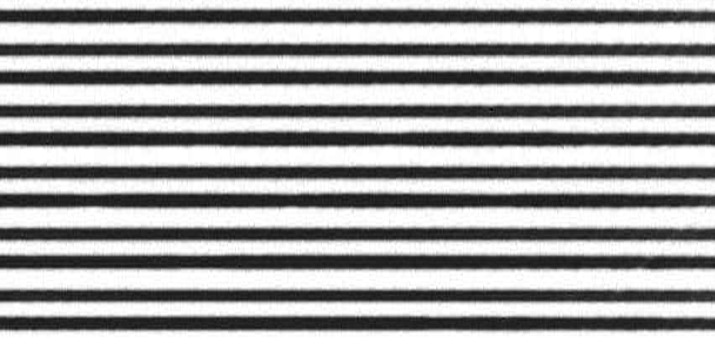
\includegraphics[angle=90,height=\figheight]{sources-validation-backpressure_0_0}
\caption{$k=0$}\label{zero_back_pressure}
\end{subfigure}
\begin{subfigure}[t]{\figwidth}\centering
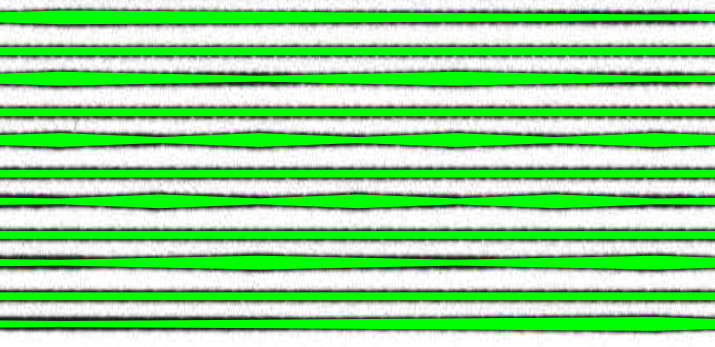
\includegraphics[angle=90,height=\figheight]{sources-validation-backpressure_1_1}
\caption{$k=1.1$}\label{back_pressure}
\end{subfigure}
\begin{subfigure}[t]{\figwidth}\centering
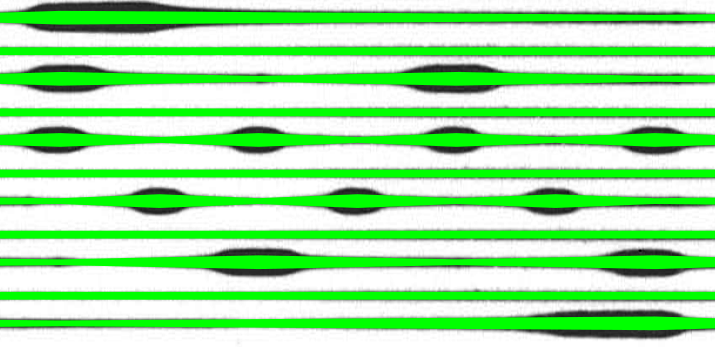
\includegraphics[angle=90,height=\figheight]{sources-validation-backpressure_2_0}
\caption{$k=2.0$}\label{too_much_back_pressure}
\end{subfigure}
\caption{
Print results (black) of the varying width test on top of a dense white raft.
Target widths in green.
\subref{zero_back_pressure} Simple flow equalization without back pressure compensation results in nearly constant bead widths.
\subref{back_pressure} A value of $k=1.1$ seems to produce good results.
}
\label{back_pressure_compensation}
\end{figure}

% discussion of print results
\todo{TODO: discuss printed results.}

% adapted from 5.5 Discussion on implications
% limitations of back pressure compensation
Our back pressure compensation method effectively changes the speed to realize adaptive width,
but this approach is limited, since the movement speed is constrained by acceleration considerations near bends in the toolpath~\cite{Ertay2018}.
Moreover, as the layer height is decreased the back pressure becomes larger compared to the internal pressure, which might cause the back pressure compensation method to demand prohibitively slow movement speeds.
%
% direct drive & pressure advance
Accurate flow control can be further enhanced by using a direct drive hardware system and by employing \emph{pressure advance algorithms} which dynamically change the internal pressure \cite{tronvoll2019investigating}.
Conversely such a setup might benefit from some form of back pressure compensation as well.


\begin{figure}
\centering
\setlength{\figwidth}{0.9\columnwidth}
\begin{subfigure}{\figwidth}\centering
%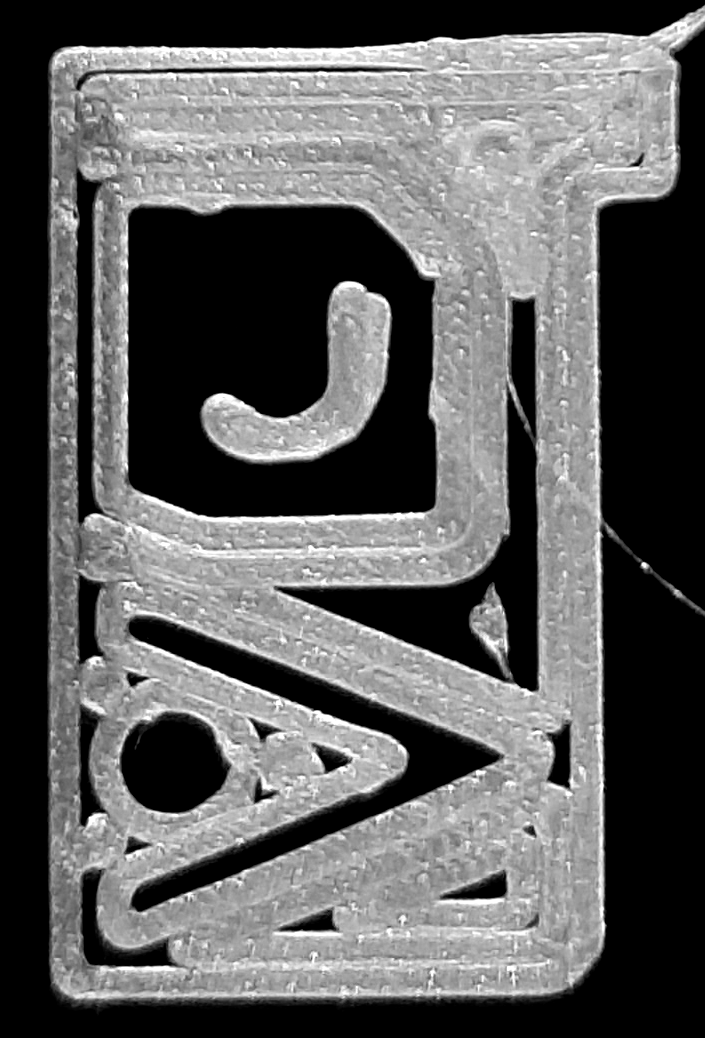
\includegraphics[height=\figheightTwo]{sources-applications-gMAT-naive.png}
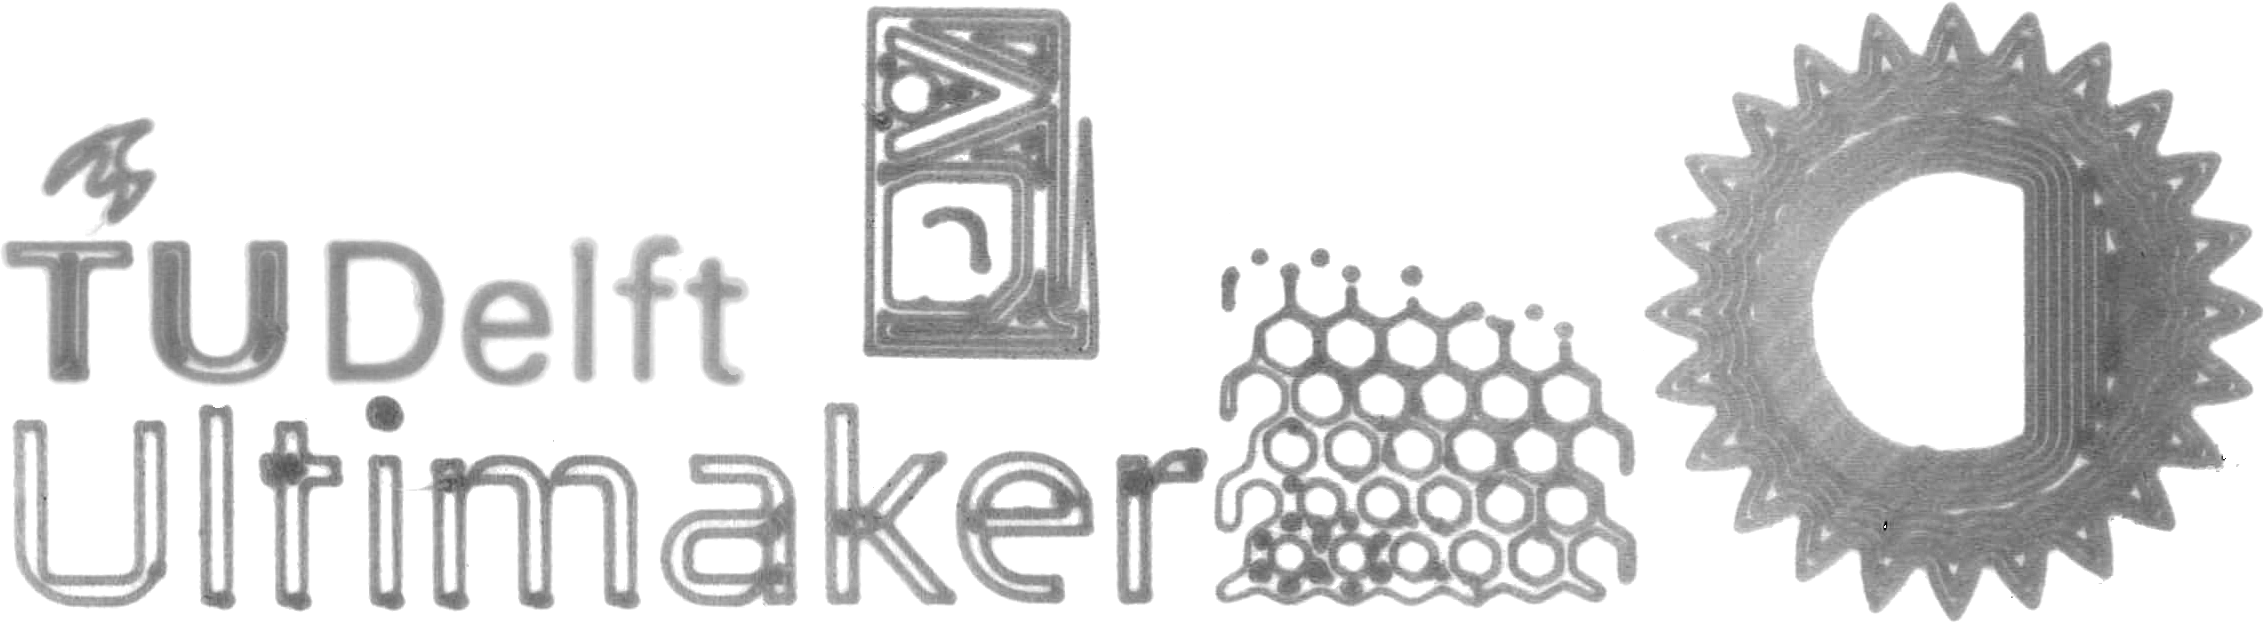
\includegraphics[width=\figwidth]{sources-applications-result-prints-naive-bw.png}
\caption{Uniform}\label{print_naive}
\end{subfigure}
\begin{subfigure}{\figwidth}\centering
%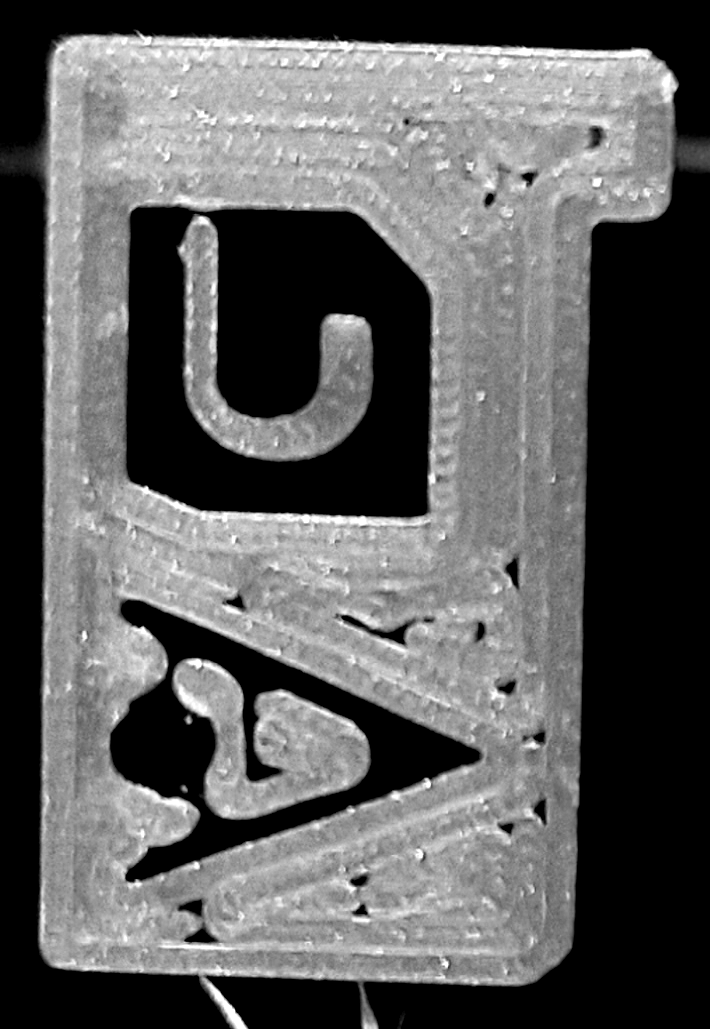
\includegraphics[height=\figheightTwo]{sources-applications-gMAT-center.png}

\includegraphics[width=\figwidth]{sources-applications-result-prints-center-bw.png}
\caption{Centered}\label{print_center}
\end{subfigure}
\begin{subfigure}{\figwidth}\centering
%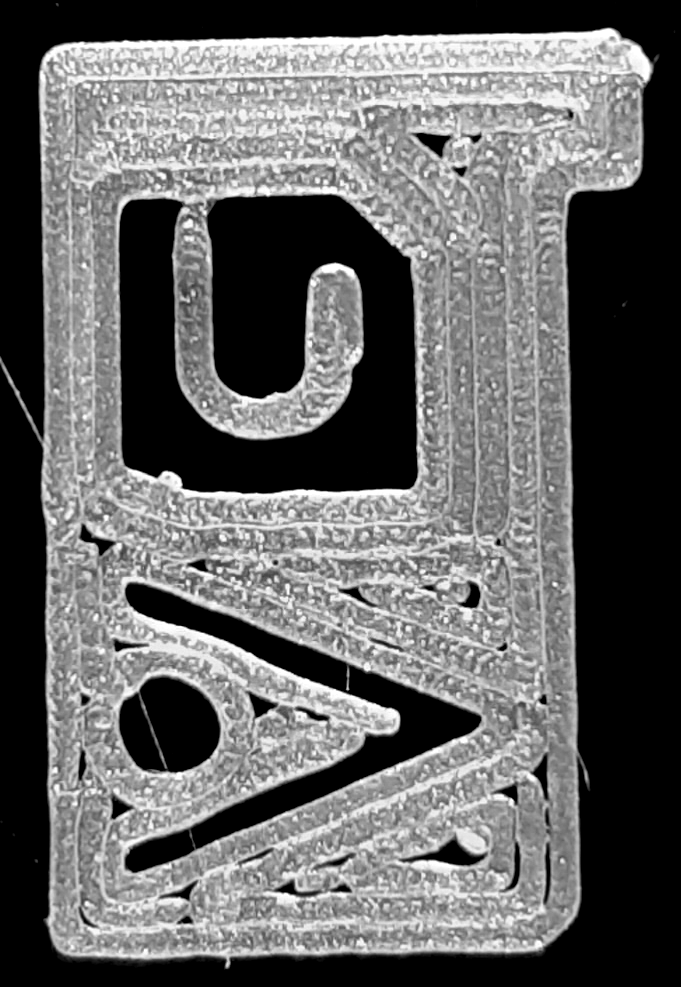
\includegraphics[height=\figheightTwo]{sources-applications-gMAT-inward.png}

\includegraphics[width=\figwidth]{sources-applications-result-prints-inward-bw.png}
\caption{Inward distributed}\label{print_inward}
\end{subfigure}
\caption{
Test shapes printed using the uniform scheme, centered scheme and the inward distributed scheme.
The uniform technique produces distinct underfill areas.
The centered scheme shows some defects due to inaccurate control of extreme deposition widths.
The inward distributed scheme produces the least defects.
}
\label{prints}
\end{figure}


}




\revise{}
{
\subsection{Computational results}\label{sec_computational_results}
} % tew
We evaluate the proposed framework and the various beading schemes on a set of different types of 3D models, ranging over various applications and various types of geometry. 
The data set is described in Appendix~\ref{dataset}.
We sliced all models in the data set and selected 300 random slices for analysis.
Toolpaths of these 300 outline shapes are generated using the uniform technique as implemented by Clipper~\cite{johnson2014clipper} -- a state-of-the-art polygon offset library,
and by our framework using four beading schemes, i.e. the constant bead count scheme with a bead count of $C=4$, the centered, the evenly distributed, and the inward distributed beading scheme using \revise{$N=3$}{$N=2$}, all with a preferred bead width\revise{s}{} of \revise{$w^* = \SI{0.4}{\milli\meter}$}{$w^* = \SI{0.5}{\milli\meter}$ and using the widening meta-scheme to enforce a minimum printed feature size of $w_\text{min}=2r_\text{min}=\SI{0.3}{\milli\meter}$}.
The tests were performed on a desktop PC equipped with an Intel Core i7-7500U CPU @ \SI{2.70}{\giga\hertz} (a single core is used) and \SI{16.3}{\giga\byte} memory.
\revise{}{We report on the total statistics summed over the whole data set, because averaging would be biased.}






\subsubsection{Accuracy}
We first evaluate the accuracy of different beading schemes in terms of the relative amount of the overfill and underfill. 
We construct the over- and underfill area by comparing the shapes covered by each extrusion move \revise{(\cref{segment_visualization_simple})}{} with each other and with the total shape of the boundary polygons. (For implementation details see Appendix~\ref{accuracy_calculation}.)
This results in polygonal shapes such as visualized in the top half of \cref{visualized_accuracy}:
there are orange shapes where the beads overlap and azure shapes in the voids in between the beads.
%
%
We compare the total area in \si{\milli\meter\squared} of these overfill and underfill shapes to the total area of the boundary for each sample in the data set
and report the average percentages in \revise{see }{}\cref{over_underfill}.
The inward distributed scheme has a calculated overfill of \revise{\SI{0.24}{\percent}}{\SI{0.30}{\percent}} and an underfill of \revise{\SI{0.17}{\percent}}{\SI{0.24}{\percent}}.
This is lower compared to the uniform scheme, which results in \revise{\SI{1.2}{\percent}}{\SI{1.63}{\percent}} overfill and \revise{\SI{1.7}{\percent}}{\SI{1.62}{\percent}} underfill in the data set.
\iffalse
names ['naive', 'Constant', 'Center', 'Distributed', 'InwardDistributed']
overfill [  1.63223926  22.21073295   0.37059604   0.45119725   0.30226112]
outer_underfill [ 0.04664107  0.03232884  0.04357603  0.03494708  0.03475748]
underfill [ 1.62009421  0.0712721   0.76886316  0.2440984   0.24461937]
\fi

\begin{figure*}
\centering
\setlength{\figwidth}{0.19\textwidth}
\setlength{\figheight}{0.283\textwidth}
\begin{subfigure}{\figwidth}\centering
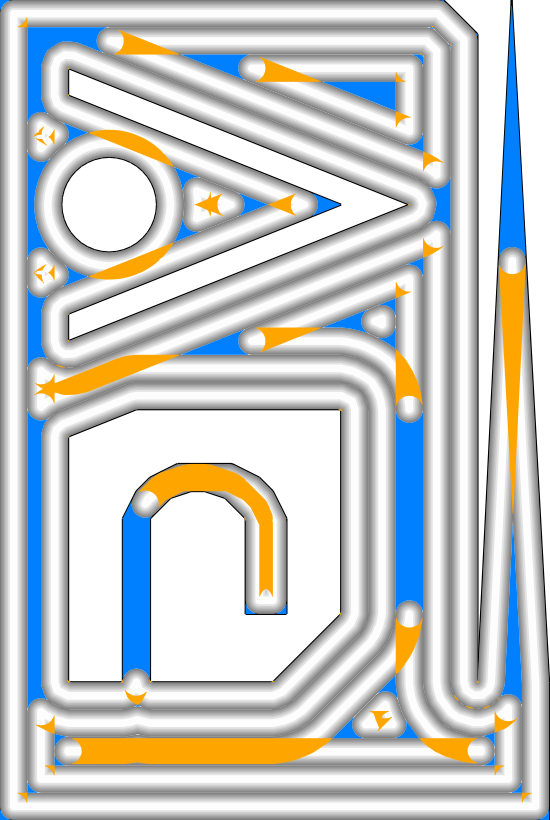
\includegraphics[height=\figheight]{sources-validation-gMAT-example-TEST-naive-accuracy.png}
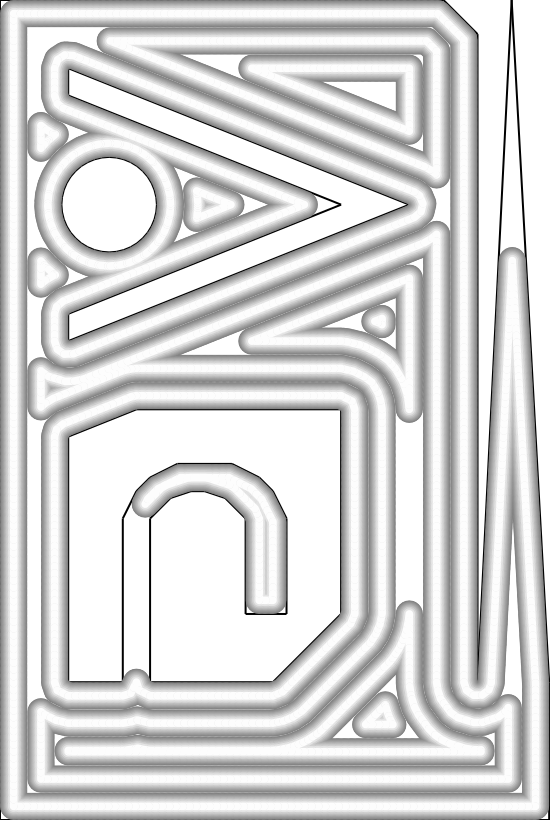
\includegraphics[height=\figheight]{sources-validation-gMAT-example-TEST-naive-widths.png}
\caption{Uniform}\label{TEST_naive_accuracy}
\end{subfigure}
%\begin{subfigure}{\figwidth}\centering
%\includegraphics[height=\figheight]{sources-validation-gMAT-example-TEST-SingleBead-accuracy.png}
%\includegraphics[height=\figheight]{sources-validation-gMAT-example-TEST-SingleBead-widths.png}
%\caption{Single}\label{TEST_SingleBead_accuracy}
%\end{subfigure}
\begin{subfigure}{\figwidth}\centering
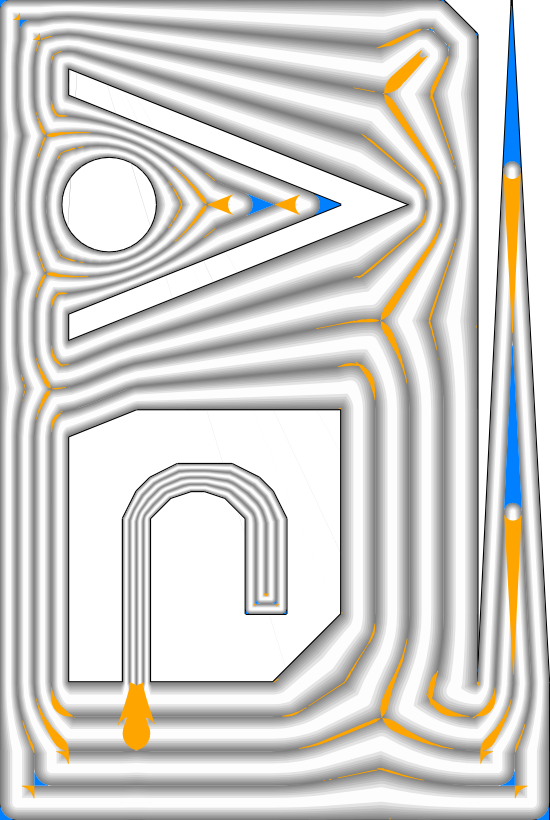
\includegraphics[height=\figheight]{sources-validation-gMAT-example-TEST-Constant-accuracy.png}
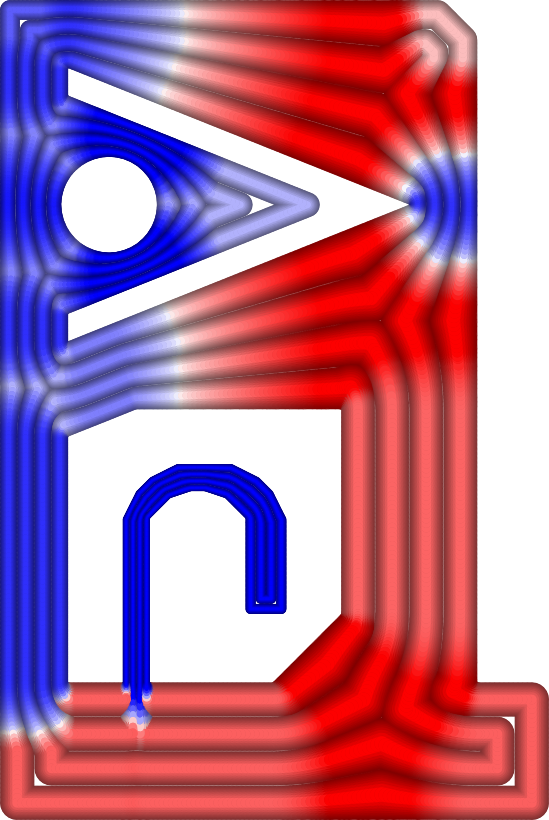
\includegraphics[height=\figheight]{sources-validation-gMAT-example-TEST-Constant-widths.png}
\caption{Constant}\label{TEST_Constant_accuracy}
\end{subfigure}
\begin{subfigure}{\figwidth}\centering
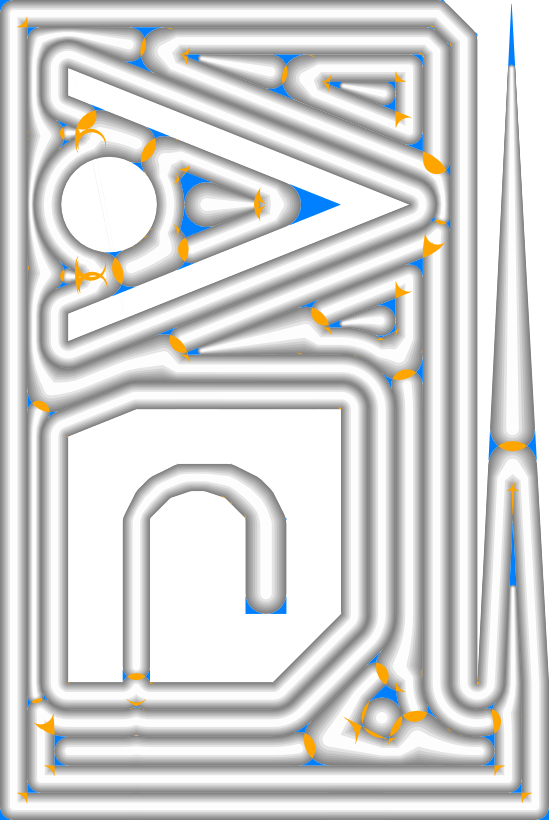
\includegraphics[height=\figheight]{sources-validation-gMAT-example-TEST-Center-accuracy.png}
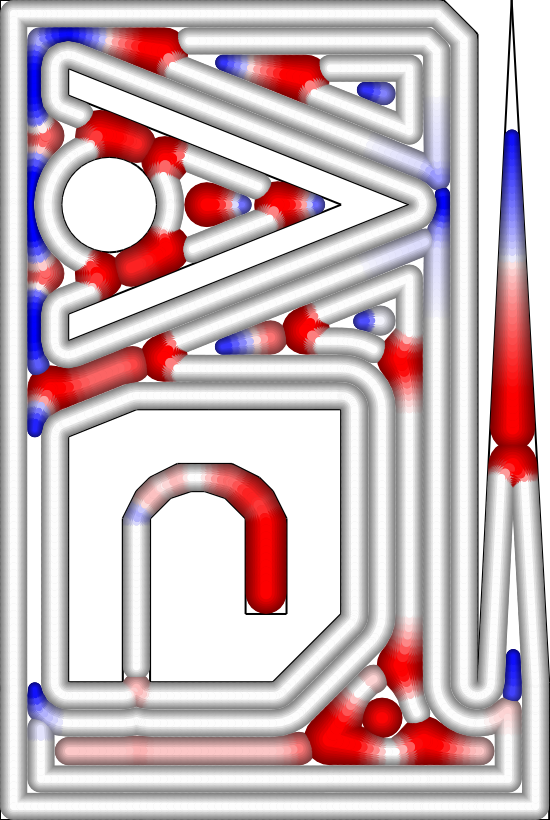
\includegraphics[height=\figheight]{sources-validation-gMAT-example-TEST-Center-widths.png}
\caption{Centered}\label{TEST_Center_accuracy}
\end{subfigure}
\begin{subfigure}{\figwidth}\centering
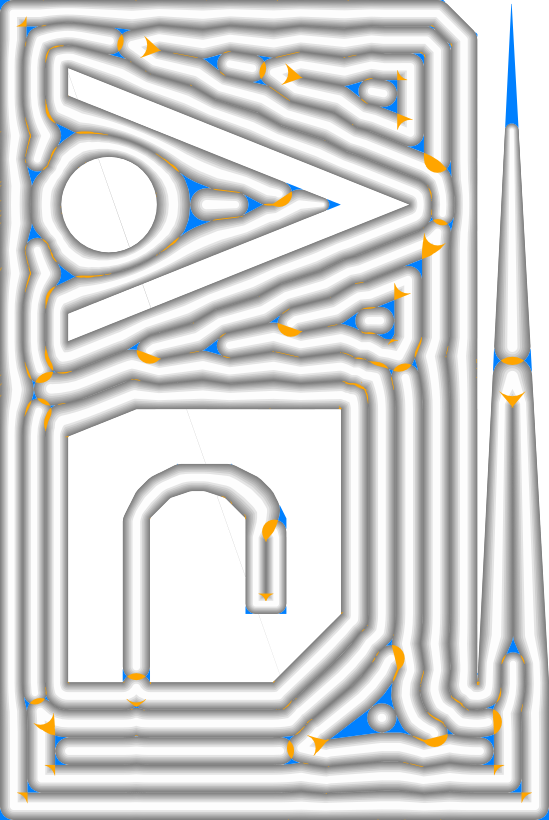
\includegraphics[height=\figheight]{sources-validation-gMAT-example-TEST-Distributed-accuracy.png}
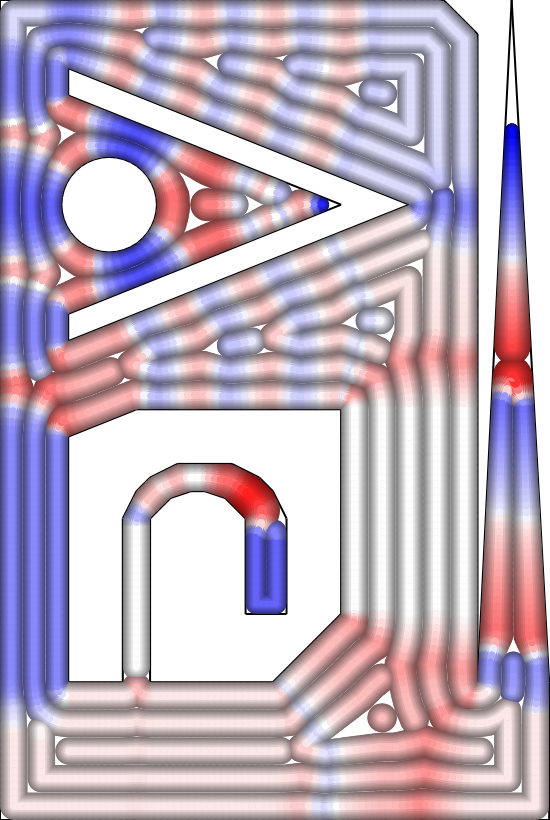
\includegraphics[height=\figheight]{sources-validation-gMAT-example-TEST-Distributed-widths.png}
\caption{Distributed}\label{TEST_Distributed_accuracy}
\end{subfigure}
\begin{subfigure}{\figwidth}\centering
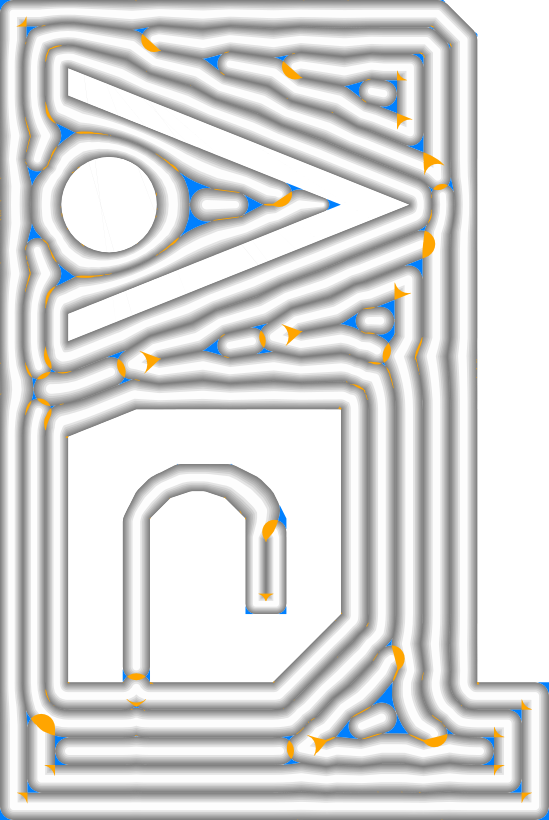
\includegraphics[height=\figheight]{sources-validation-gMAT-example-TEST-InwardDistributed-accuracy.png}
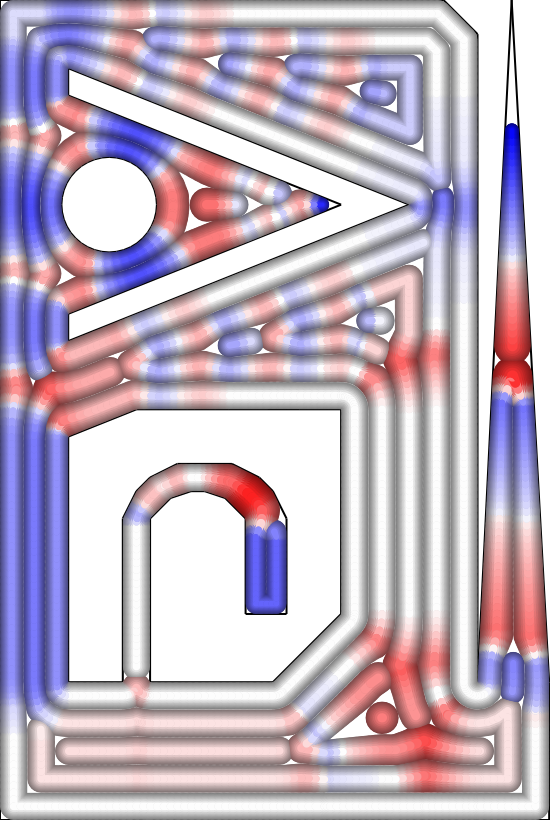
\includegraphics[height=\figheight]{sources-validation-gMAT-example-TEST-InwardDistributed-widths.png}
\caption{Inward \revise{}{($N=2$)}}\label{TEST_InwardDistributed_accuracy}
\end{subfigure}
\begin{subfigure}{.04\columnwidth}\centering
\vspace{4.7cm}
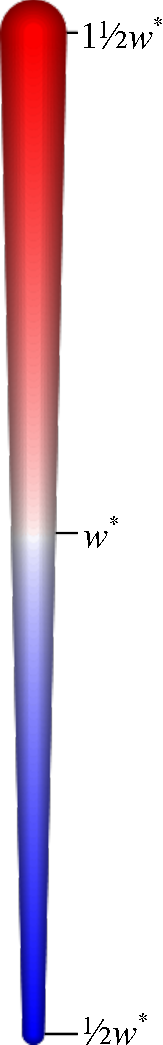
\includegraphics[height=\figheight]{sources-validation-gMAT-example-widths-legend.pdf}
\end{subfigure}
\caption{
Visualization of the overfills and underfills (top) and the widths (bottom) for various beading schemes.
Extrusion beads in gray tones,
overfill in orange,
underfill in azure,
narrow beads in blue
and wide beads in red.
\revise{New shape contains pointy wedge to see impact on minimal feature size}{In order to distinguish clearly from the Distributed scheme the Inward is limited to $N=2$.}
}
\label{visualized_accuracy}
\end{figure*}




\begin{figure*}
\centering
\setlength{\figheight}{0.25\textwidth}
\setlength{\figwidth}{0.32\textwidth}
\begin{subfigure}{\figwidth}\centering
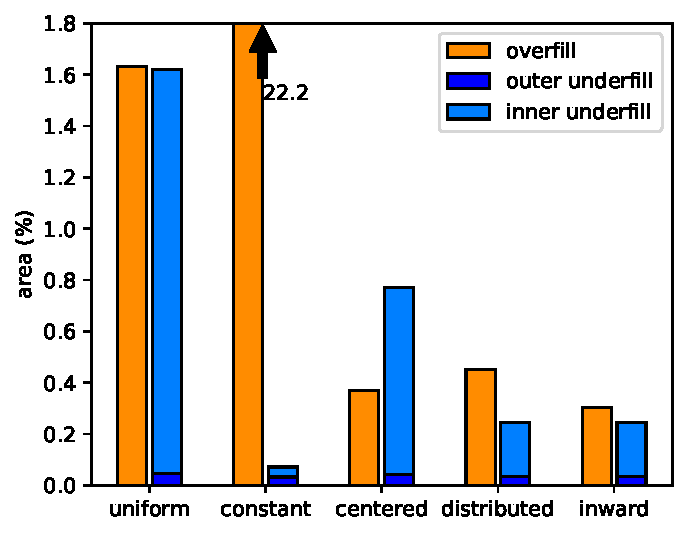
\includegraphics[height=\figheight]{sources-validation-over-underfill.pdf}
%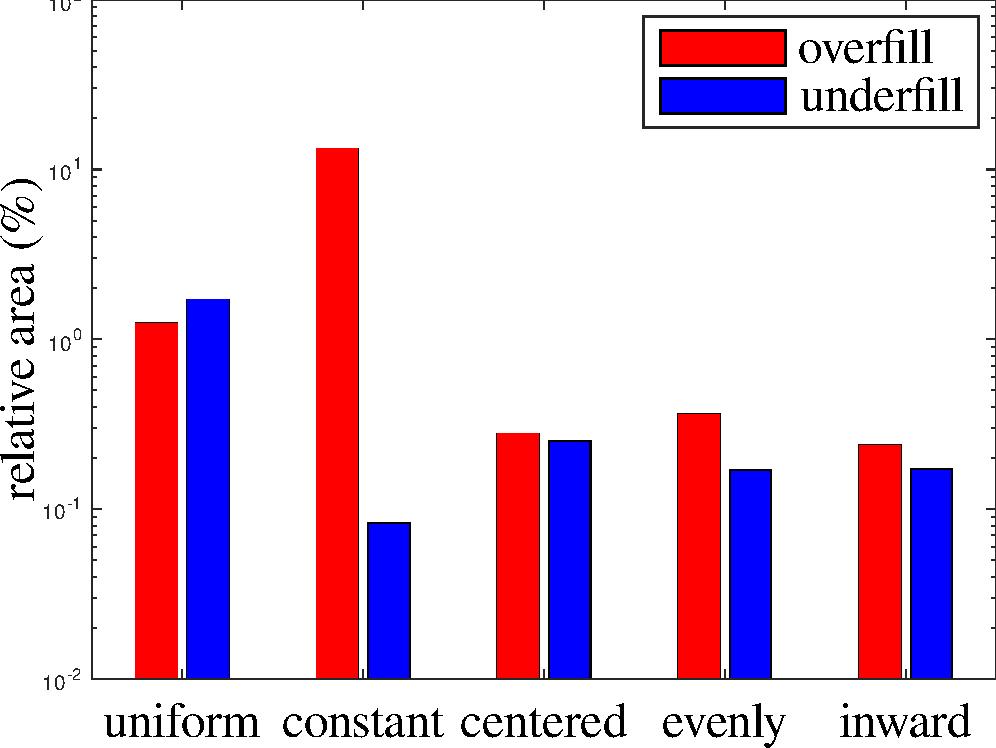
\includegraphics[width=\figwidth]{sources-validation-overunderfill.pdf}
\caption{\revise{}{Over- and underfill}}
\label{over_underfill}
\end{subfigure}
\begin{subfigure}{\figwidth}\centering
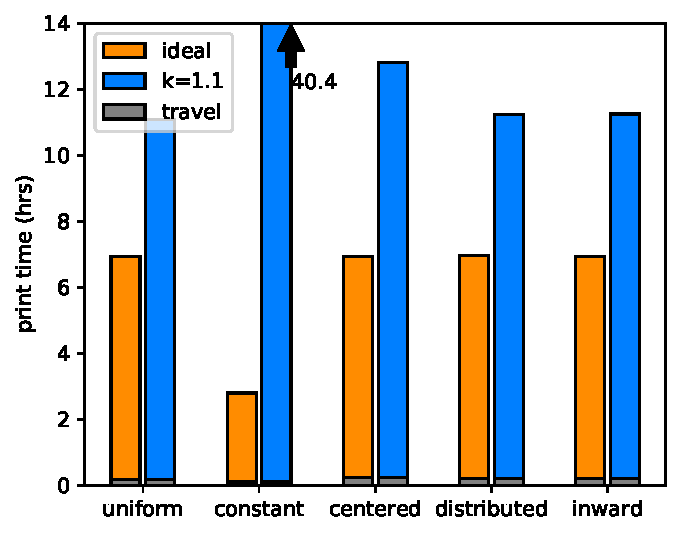
\includegraphics[height=\figheight]{sources-validation-print-time.pdf}
%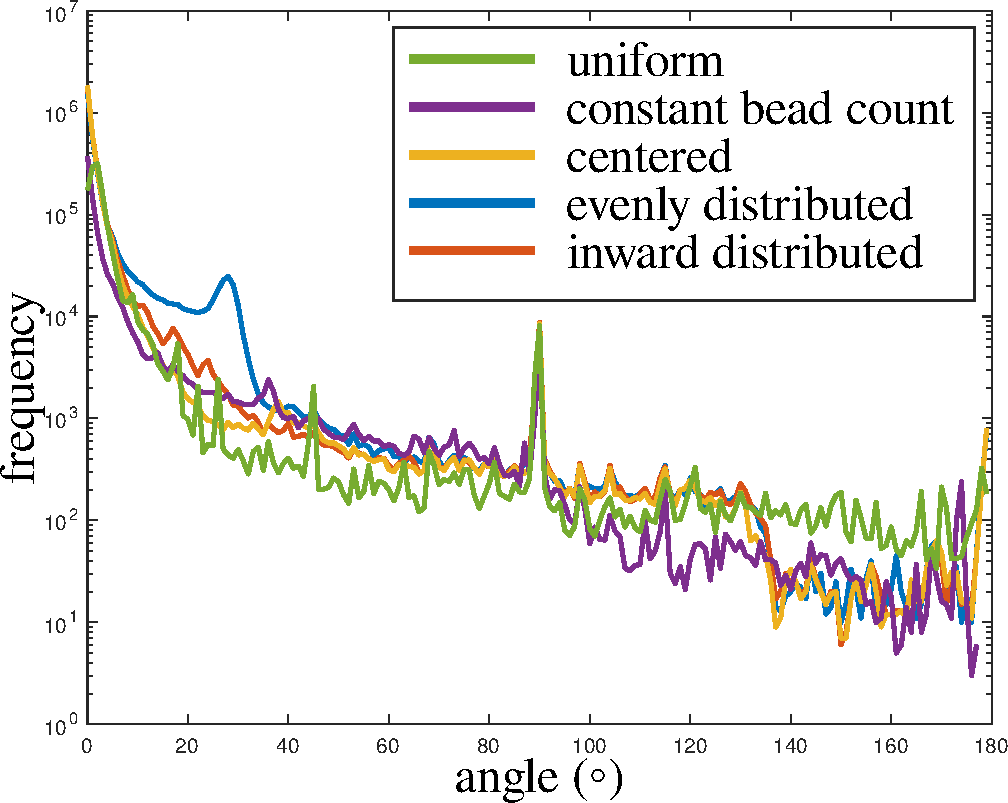
\includegraphics[width=\figwidth]{sources-validation-smoothness.pdf}
\caption{\revise{}{Print time}}
\label{printtime}
\end{subfigure}
\begin{subfigure}{\figwidth}\centering
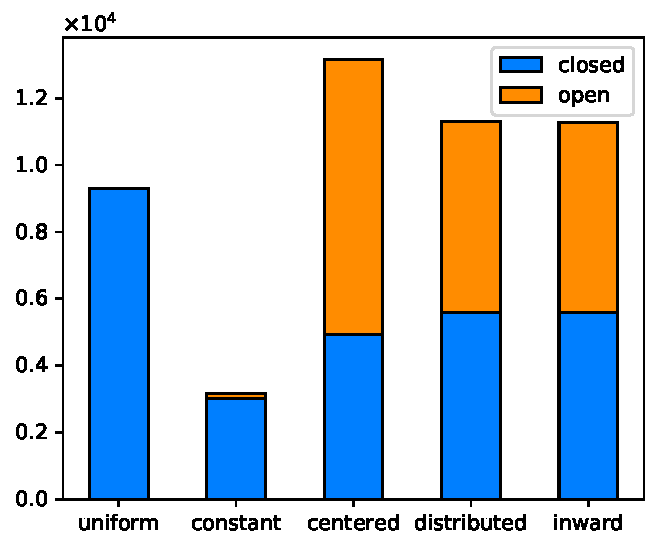
\includegraphics[height=\figheight]{sources-validation-path-counts.pdf}
%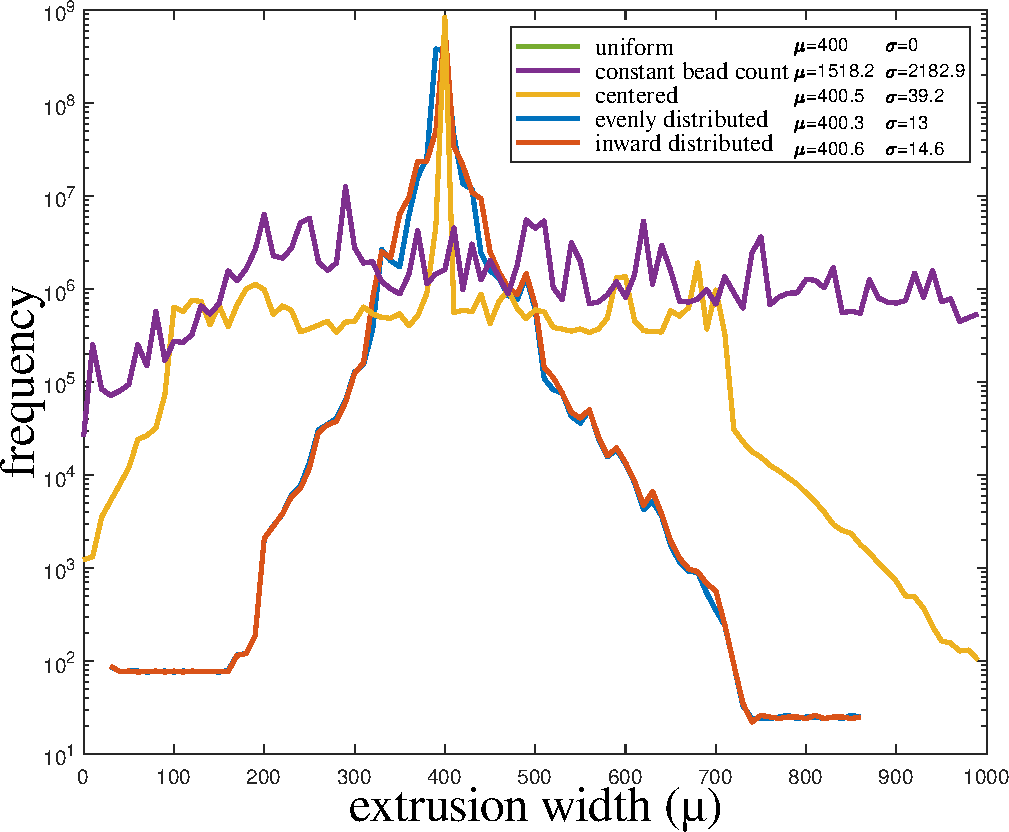
\includegraphics[width=\figwidth]{sources-validation-widthHistogram.pdf}
\caption{\revise{}{Path counts}}
\label{pathcounts}
\end{subfigure}

\begin{subfigure}{\figwidth}\centering
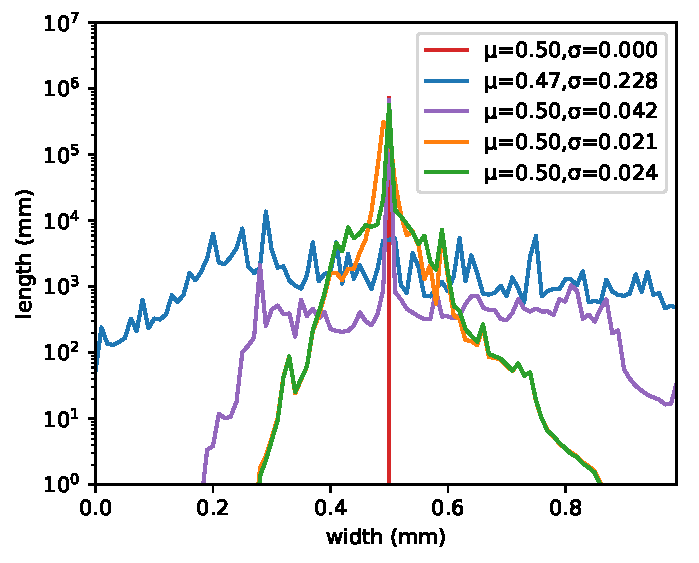
\includegraphics[height=\figheight]{sources-validation-widths.pdf}
%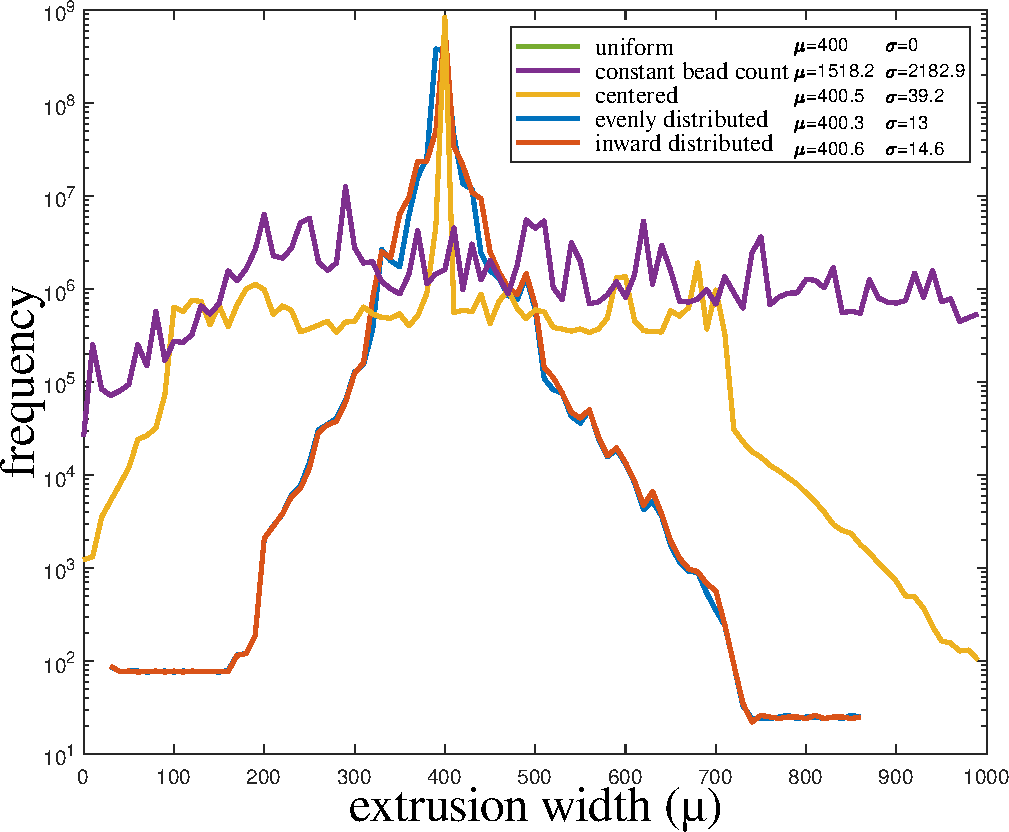
\includegraphics[width=\figwidth]{sources-validation-widthHistogram.pdf}
\caption{\revise{}{Extrusion widths}}
\label{widthHistogram}
\end{subfigure}
\begin{subfigure}{\figwidth}\centering
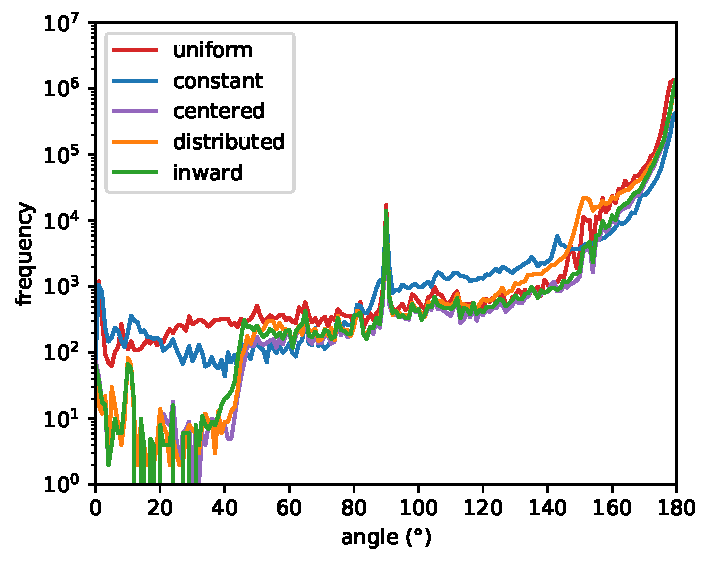
\includegraphics[height=\figheight]{sources-validation-angles.pdf}
%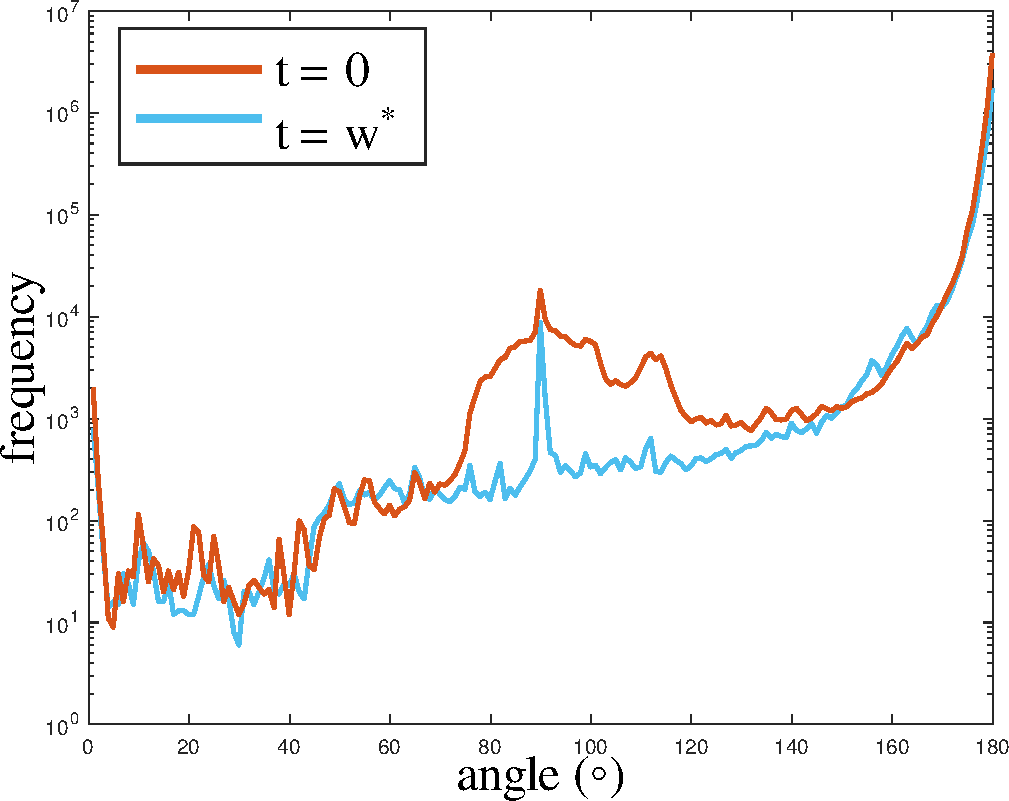
\includegraphics[width=\figwidth]{sources-validation-smoothnessNoTransition.pdf}
\caption{\revise{}{Site angles}}
\label{smoothness}
\end{subfigure}
\begin{subfigure}{\figwidth}\centering
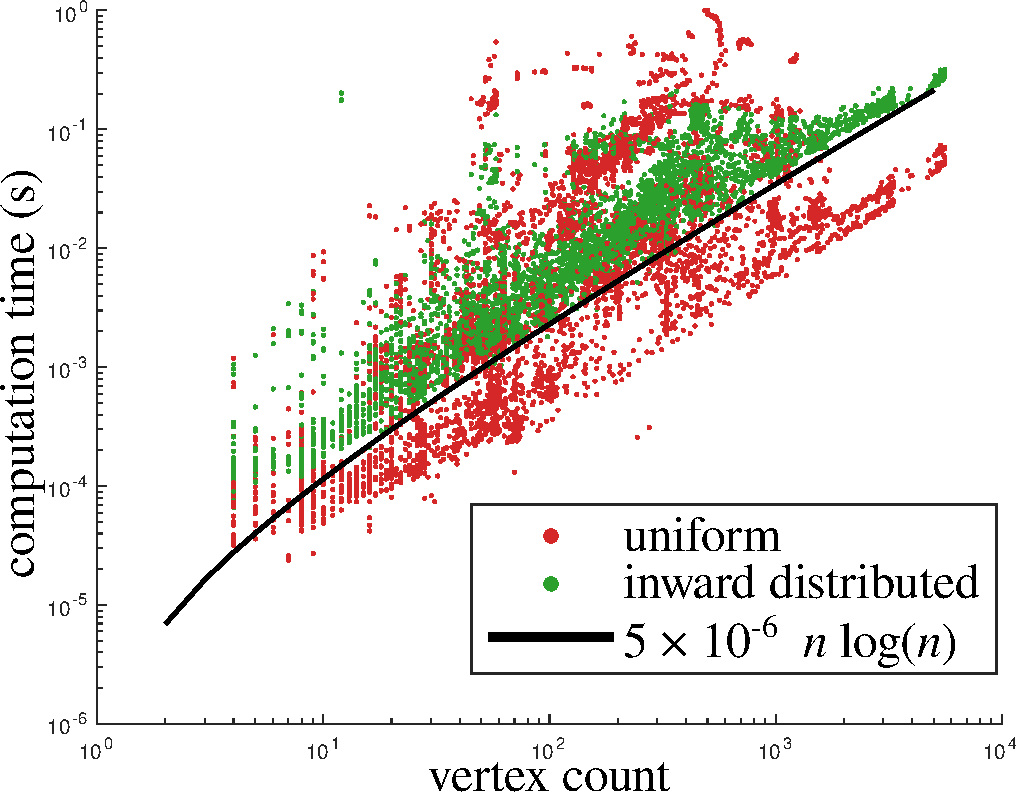
\includegraphics[height=\figheight]{sources-validation-computime2.pdf}
%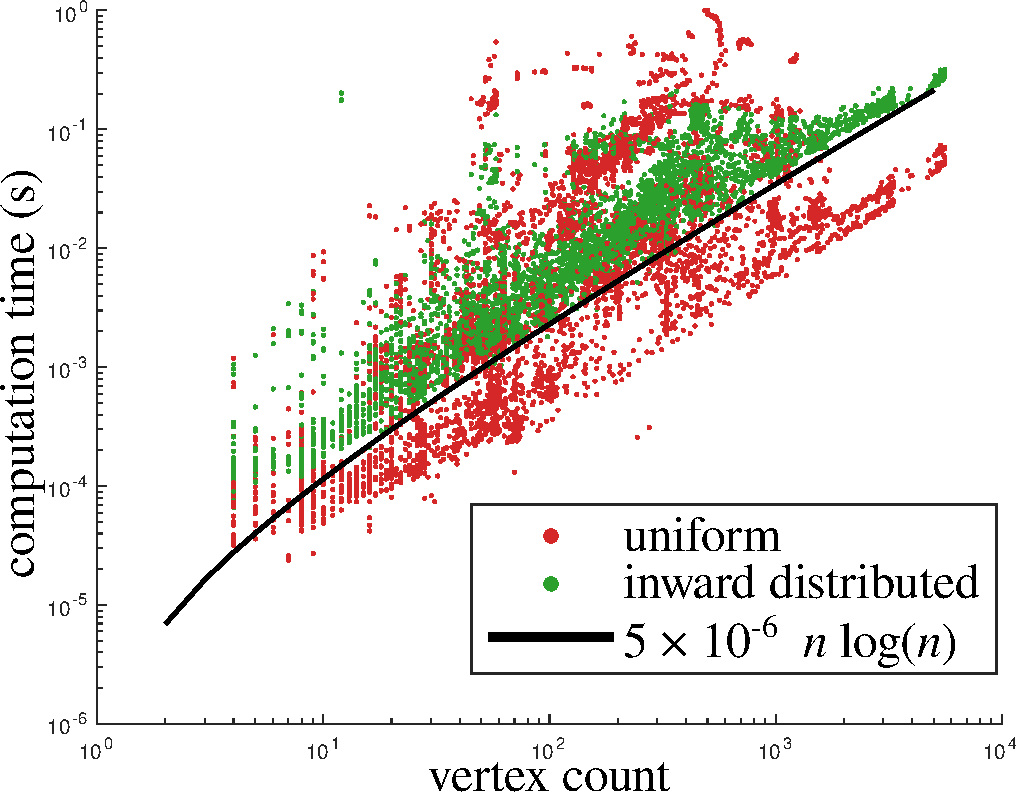
\includegraphics[width=\figwidth]{sources-validation-computime2.pdf}
\caption{Computation time}
\label{computime}
\end{subfigure}


\caption{
Statistical analysis of the toolpaths from applying the uniform width technique and various beading schemes using our framework to a data set of 300 slices.
Note the use of a logarithmic scale \revise{}{in the bottom graphs }on the Y-axes and \revise{on some of}{for \subref{computime} on} the X-axes as well.
}
\label{statisticsfig}
\end{figure*}







\subsubsection{Uniformity}
We visualize the bead widths resulting from the different schemes in the bottom of \cref{visualized_accuracy}.
\revise{
We calculated the mean and standard deviation of the bead width, sampled at \SI{1}{\micro\meter} along the toolpaths.
\cref{widthHistogram} shows the distribution of extrusion width for each scheme binned at intervals of \SI{10}{\micro\meter}.
}{
We binned the toolpaths into width bins at \SI{0.01}{\milli\meter} increments and determine the total toolpath length pertaining to each bin.
From these statistics we calculate the mean and standard deviation and report them in \cref{widthHistogram}.
}
We found that the mean width of the inward and evenly distributed schemes is close to \revise{}{the }preferred bead width of \revise{\SI{400}{\micro\meter}}{\SI{0.5}{\milli\meter}}, while their standard deviation is lower than for the centered and constant bead count scheme. 
These results show that, while causing less overfill and underfill, inwards distributed and evenly distributed schemes deviate less or less often from the preferred bead width compared to the other schemes.
\revise{
We compared the width uniformity of the 6 outer beads for the inward and evenly distributed schemes, the distribution of these extrusion widths is shown in \cref{widthIndexedHistogram}. 
The outer beads of the inward distributed scheme deviate less from the preferred width compared to the evenly distributed scheme.
}{}

\revise{
\subsubsection{Smoothness of toolpaths}
In order to maintain a high printing speed, it is desirable that toolpaths have fewer and less sharp corners. 
We therefore measured the angle between consecutive extrusion segments generated by each scheme
and report on the occurrence of each angle in \cref{smoothness}.
All schemes show a higher number of corners for smaller angles with a peak towards \SI{180}{\degree} (straight).
We observe that compared to the uniform method our framework produces less acute angles which, but more obtuse angles.
The inward distributed scheme produces an order of magnitude less corners around \SI{150}{\degree}, compared to evenly distributed. 
We also investigated the effect of the transition regions on the smoothness of the toolpaths. 
\cref{smoothnessNoTransition} shows that introducing the transitions greatly reduces the number of corners around \SI{90}{\degree}. 
}{
\subsubsection{Print time}
The total time it takes to print a part is influenced not only by our back pressure compensation scheme, but also by the geometry of the toolpaths.
In order to separate these effects we report on the total print time when using back pressure compensation and when using a constant (maximum) movement speed in \cref{printtime}.
We estimate print times using a simulation of the Marlin firmware using the default movement settings of the setup described in \cref{print_results_section}.
While the idealized print time is predominantly determined by the total toolpath length, the print time using back pressure compensation is predominantly determined by the occurrence of wide beads, because they have a reduced the flow in \si{\milli\meter\cubed\per\second}.
Because of acceleration constraints imposed by the hardware the maximum movement speed is not reached near sharp corners.
We therefore also report on the angles of the bends in the toolpaths in \cref{smoothness}.
Furthermore, the print time is negatively affected by discontinuities in the extrusion process.
Between extrusions the printer needs to stop extrusion, travel to the next extrusion path and restart the extrusion process, which may introduce defects and incurs extra print time.
For closed polygonal toolpaths we can start anywhere within the path, so we can optimize the starting location so as to minimize the travel time.
We therefore report both on the open and closed path count in \cref{pathcounts}.
}


\subsubsection{Computational performance}
\cref{computime} plots the computation time against the vertex count of the layer for the full data set, comparing the uniform technique implemented using Clipper~\cite{johnson2014clipper} to our framework with the inward distributed scheme.
For polygonal shapes with as many as $10^4$ vertices, the computation for both approaches is less than 1 second, with our method being approximately five times that of the uniform technique.
These results could be improved upon by utilizing the locality inherent in our algorithms for parallelization on the GPU.

The computational complexity is limited by the generation of the Voronoi Diagram, which is $O(n \log n)$, where $n$ is the number of vertices in the input shape.
The other steps in our framework have a complexity of $O(m)$, where $m$ is the number of elements in the ST.
Therefore, the total running time of our algorithm is $O(n \log n)$.
Results in \cref{computime} confirm that both our framework and the uniform technique have an expected running time of approximately $5 \times 10^{-6} n \log n$ seconds.





\revise{
Test prints were performed on a custom FDM hardware setup, with a standard \SI{0.4}{\milli\meter} nozzle and a filament extrusion drive directly mounted on the print head.
The firmware of the printer employs \emph{linear advance} for accurately realizing adaptive deposition width:
gaining the extra pressure required to change to a wider bead is realized by 'advancing' an extra amount of filament into the physical system~\cite{tronvoll2019investigating}.
We set the preferred width to $w^* = \SI{0.6}{\milli\meter}$, to avoid fluttered printing of lines narrower than the nozzle size.
We used a layer thickness of \SI{0.2}{\milli\meter} and a movement speed of \SI{10}{\milli\meter\per\second}.

The prints are shown in \cref{prints}.
Because of inaccuracies in the deposition control system some of the prints show defects.
Such defects are less prevalent for the inward distributed beading scheme than the other schemes.
The prints which employ the uniform offsets technique show a lot of underfill, which impacts the visual quality of the print.
Moreover, in the case of the regular honeycomb there are several fully disconnected hexagons, which means the object falls apart.
The difference between the centered and the inward distributed schemes is less pronounced.
We can still see some loosely connected extrusion segments in both, which is attributable to inaccuracies in the extrusion system.
However, the middle of \cref{wedge_print} exhibits more defects in the regions where the centered scheme produces extreme bead widths.
The bottom print shows that the inward distributed beading scheme produces smoother prints with less defects.


\begin{figure}
\centering
\begin{subfigure}{\columnwidth}\centering
\setlength{\figwidth}{\columnwidth}
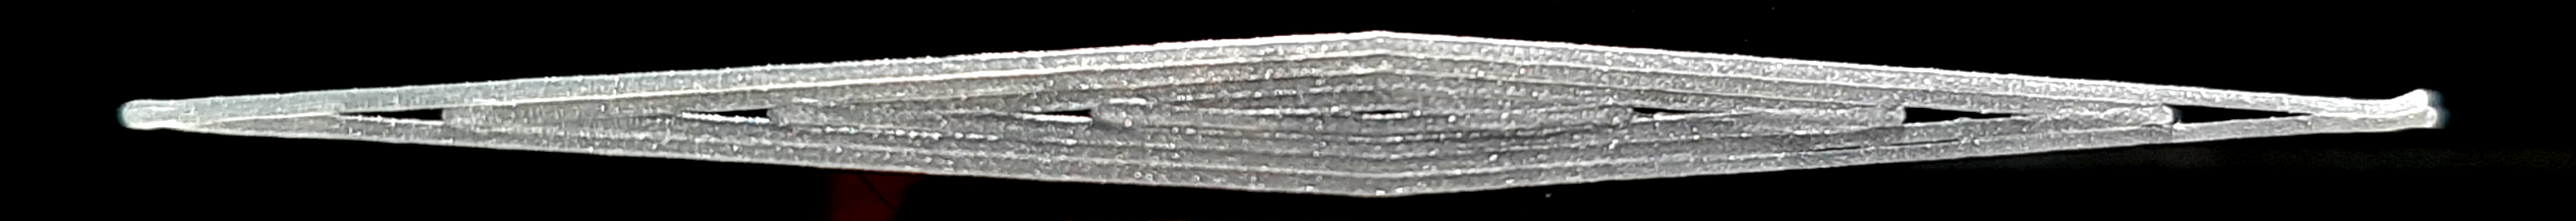
\includegraphics[width=\figwidth]{sources-applications-P3-print-wedge-naive-edited.png}
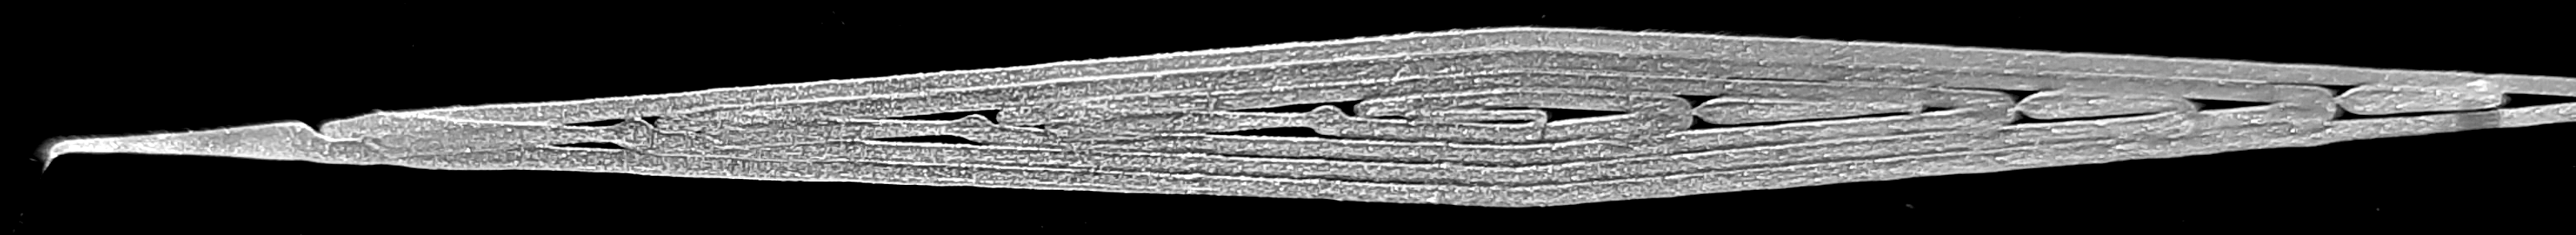
\includegraphics[width=\figwidth]{sources-applications-P3-print-wedge-center-edited.png}
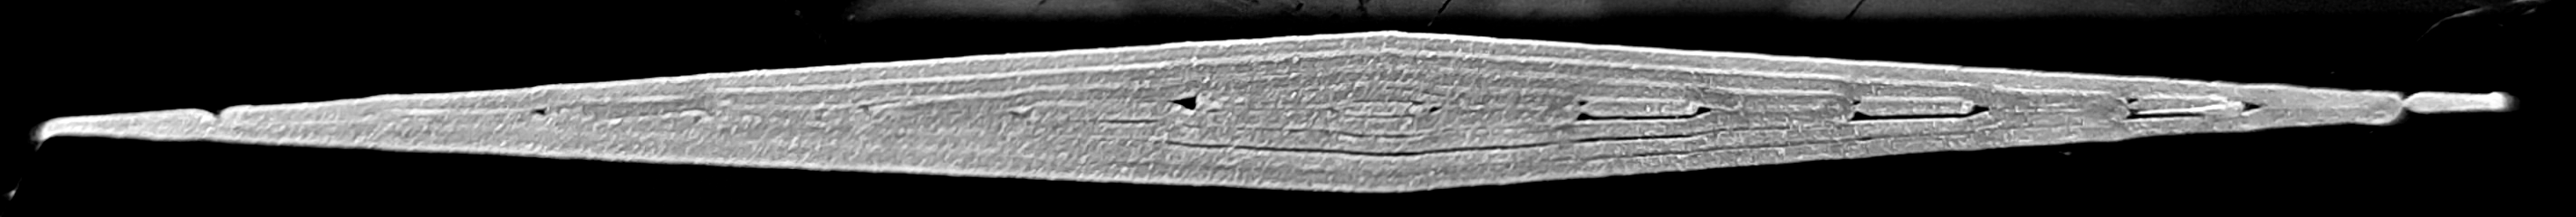
\includegraphics[width=\figwidth]{sources-applications-P3-print-wedge-inward-edited.png}
\caption{Uniform (top), centered (mid) and inward distributed (bottom)}\label{wedge_print}
\end{subfigure}
\setlength{\figheight}{.38\columnwidth}
\setlength{\figheightTwo}{.47\columnwidth}
\setlength{\figwidth}{0.32\columnwidth}
\begin{subfigure}{\figwidth}\centering
%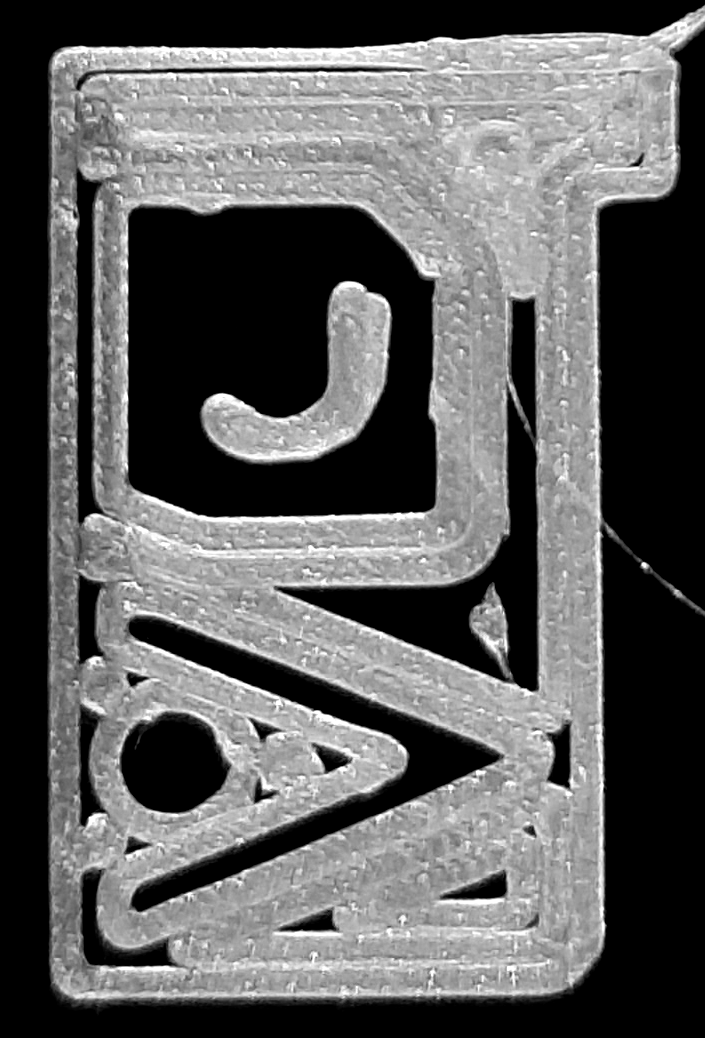
\includegraphics[height=\figheightTwo]{sources-applications-gMAT-naive.png}
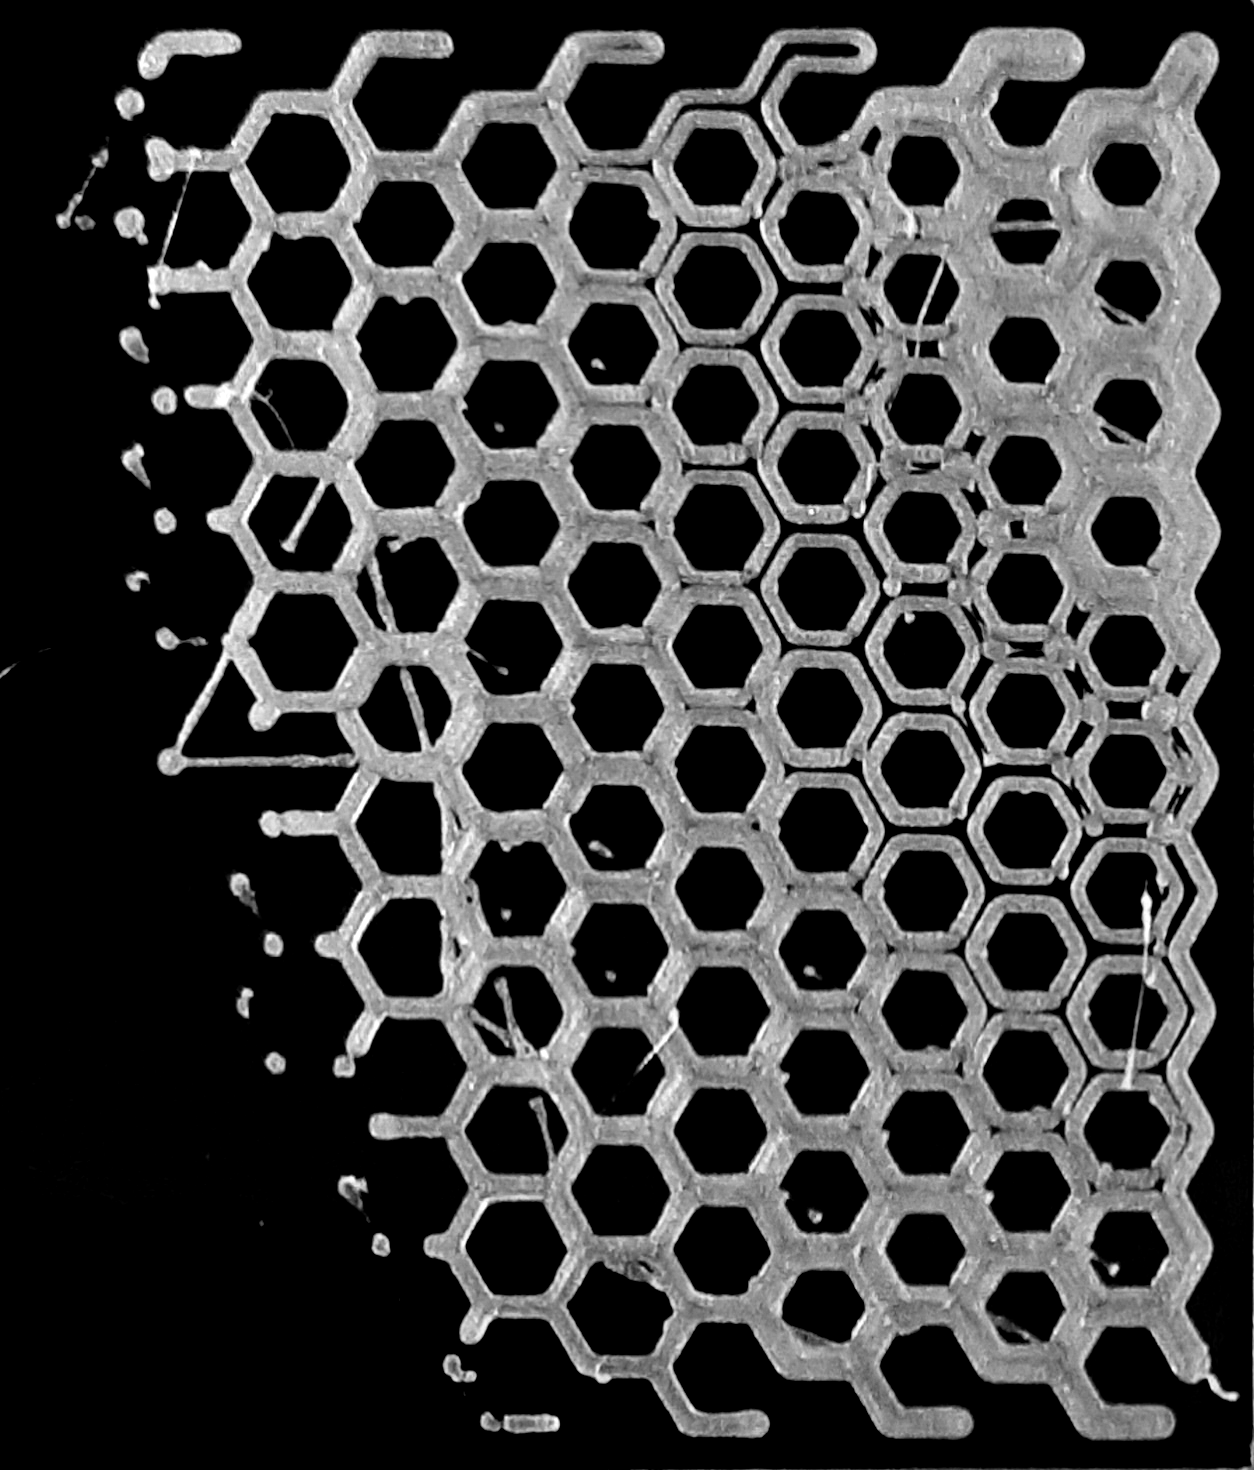
\includegraphics[height=\figheight]{sources-applications-P3-print-hex-naive-edited.png}

\includegraphics[width=\figwidth]{sources-applications-P3-print-UM-naive-edited.png}
\caption{Uniform}\label{print_naive}
\end{subfigure}
\begin{subfigure}{\figwidth}\centering
%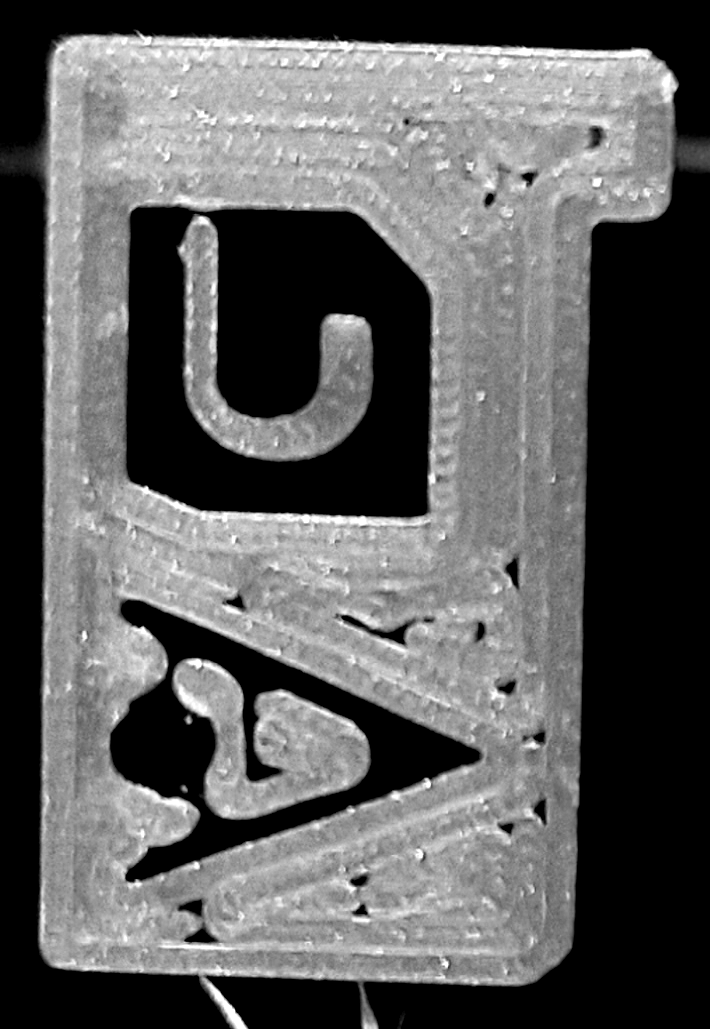
\includegraphics[height=\figheightTwo]{sources-applications-gMAT-center.png}
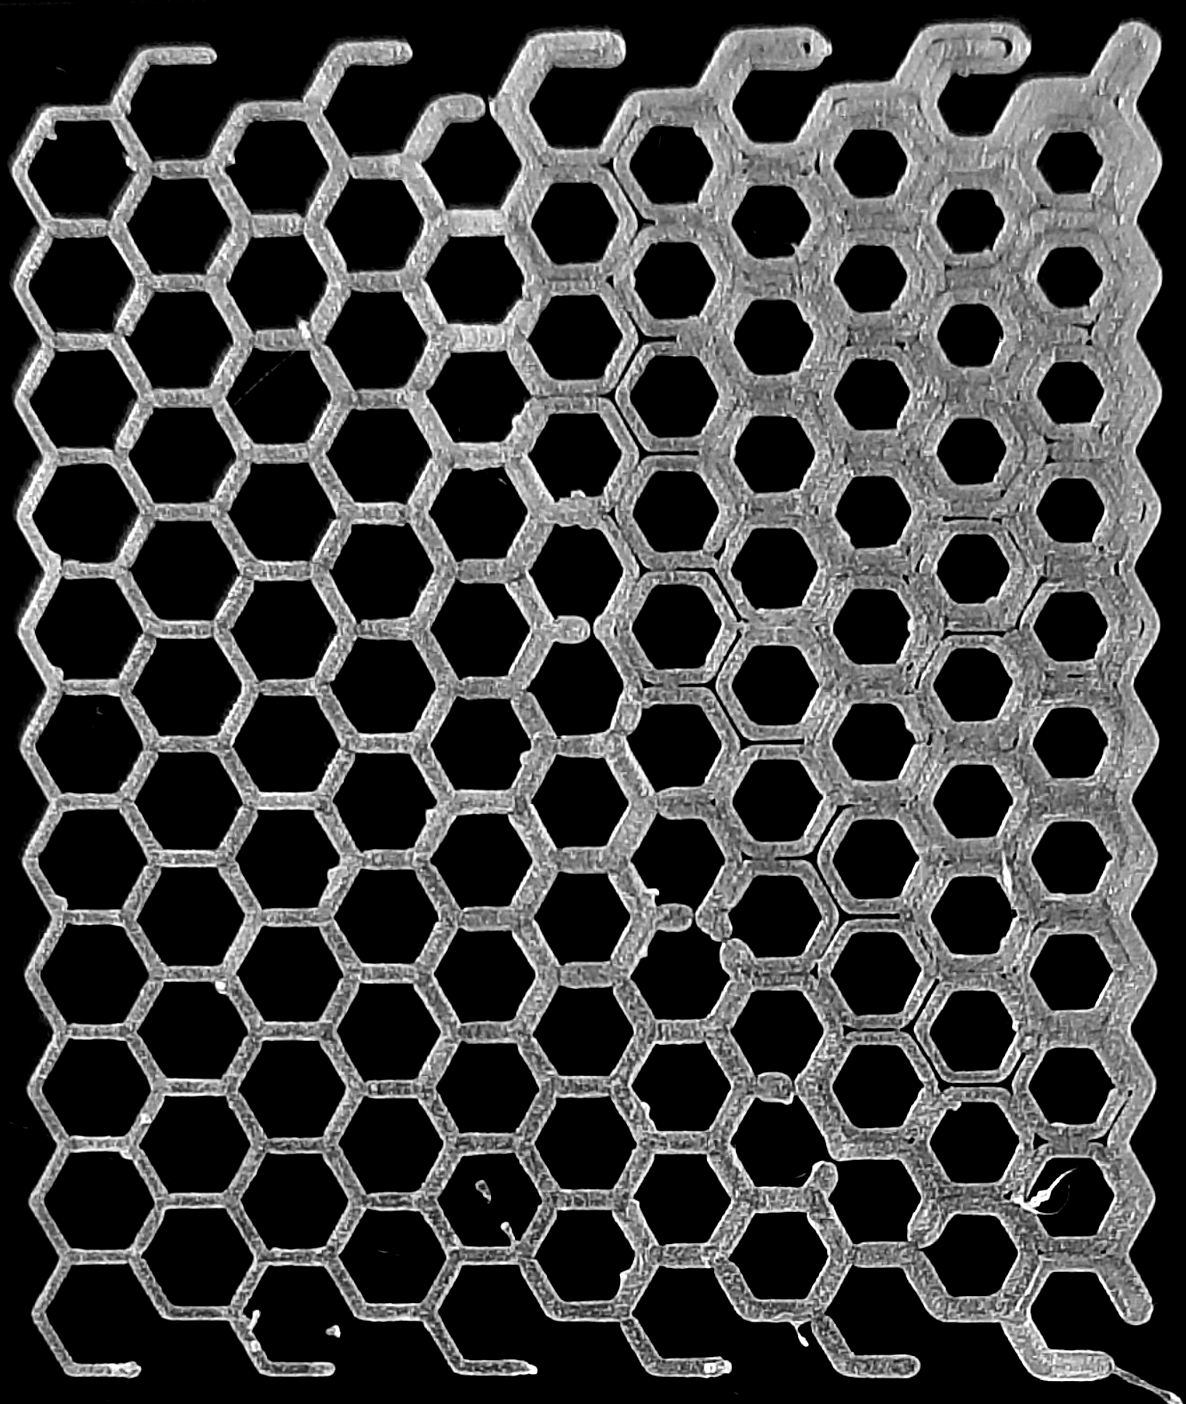
\includegraphics[height=\figheight]{sources-applications-P3-print-hex-center-edited.png}

\includegraphics[width=\figwidth]{sources-applications-P3-print-UM-center-edited.png}
\caption{Centered}\label{print_center}
\end{subfigure}
\begin{subfigure}{\figwidth}\centering
%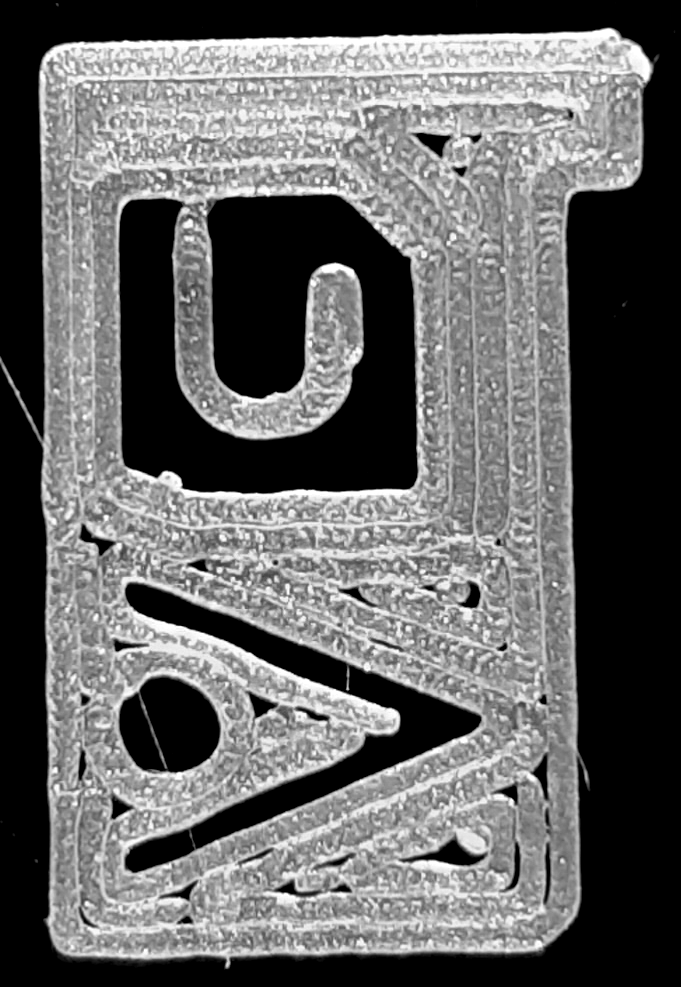
\includegraphics[height=\figheightTwo]{sources-applications-gMAT-inward.png}
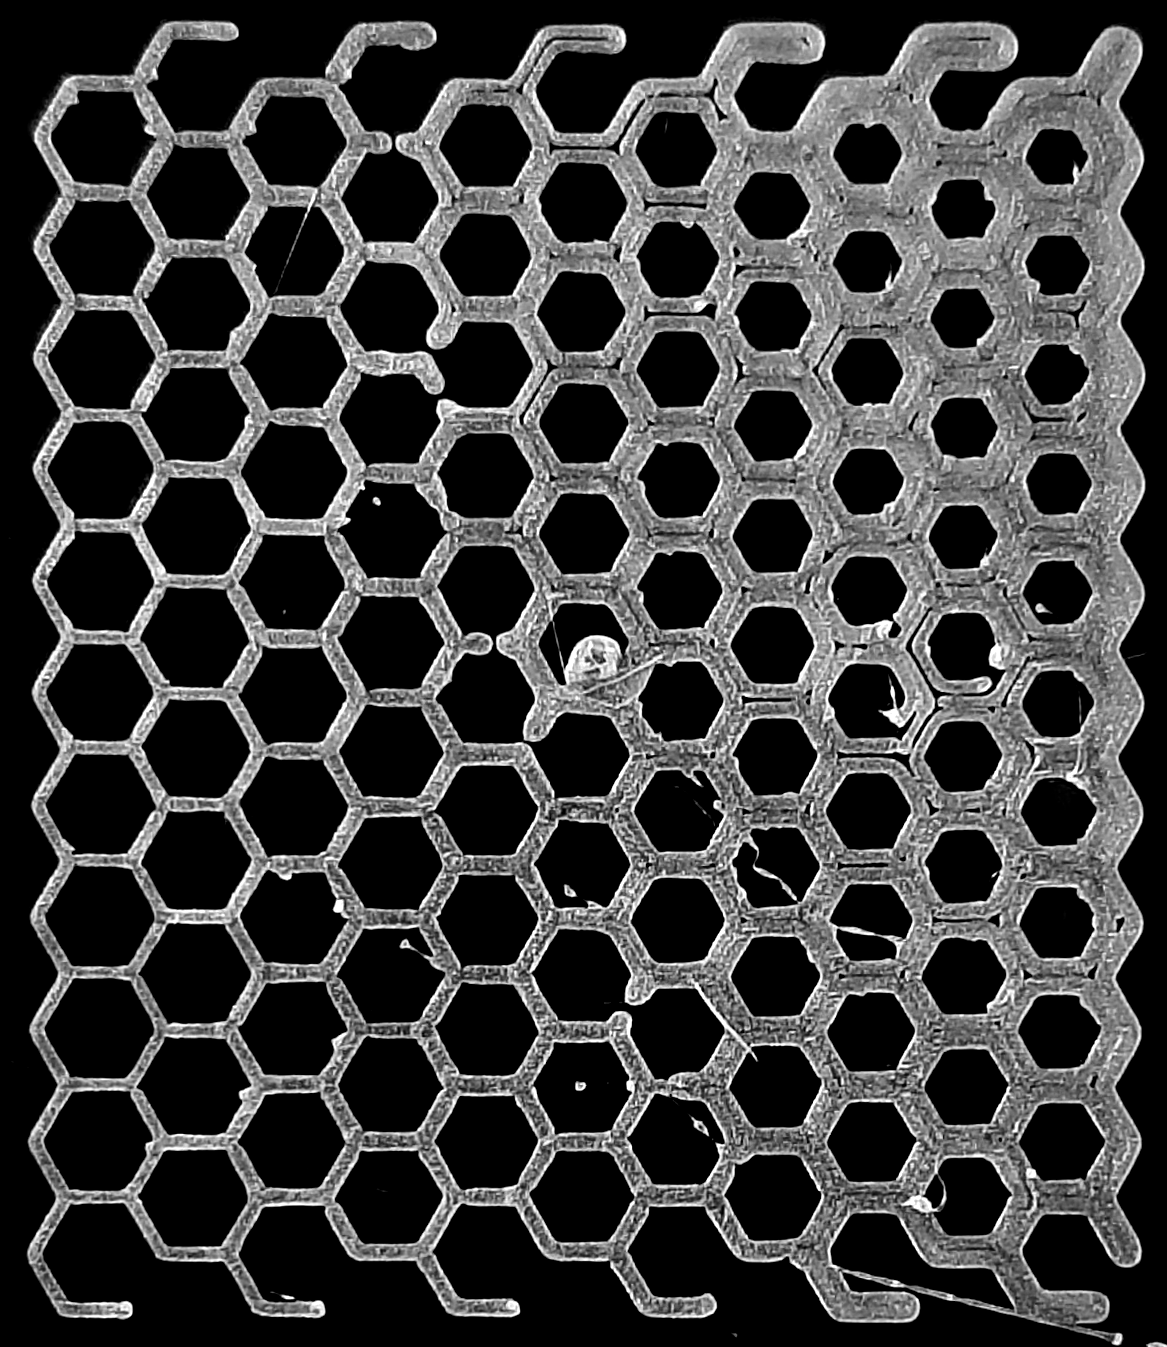
\includegraphics[height=\figheight]{sources-applications-P3-print-hex-inward-edited.png}

\includegraphics[width=\figwidth]{sources-applications-P3-print-UM-inward-edited.png}
\caption{Inward distributed}\label{print_inward}
\end{subfigure}
\caption{
Test shapes printed using the uniform scheme, centered scheme and the inward distributed scheme.
The uniform technique produces distinct underfill areas.
The centered scheme shows some defects due to inaccurate control of extreme deposition widths.
The inward distributed scheme produces the least defects.
}
\label{prints}
\end{figure}
}{}









%We therefore visualize include a semi-circle with a diameter equal to the starting width in the one end, and exclude it at the other end, because it will be included in the next extrusion segment.


